\chapter{Calculating Temperature Changes using the fMRI BOLD Response}

\section{Background}
  % What does the BOLD response tell us?
  % What gives rise to the fMRI BOLD response?
  \subsection{Generation of the {B}lood {O}xygen {L}evel {D}ependent ({BOLD}) Response}
    \begin{figure}
      \begin{center}
        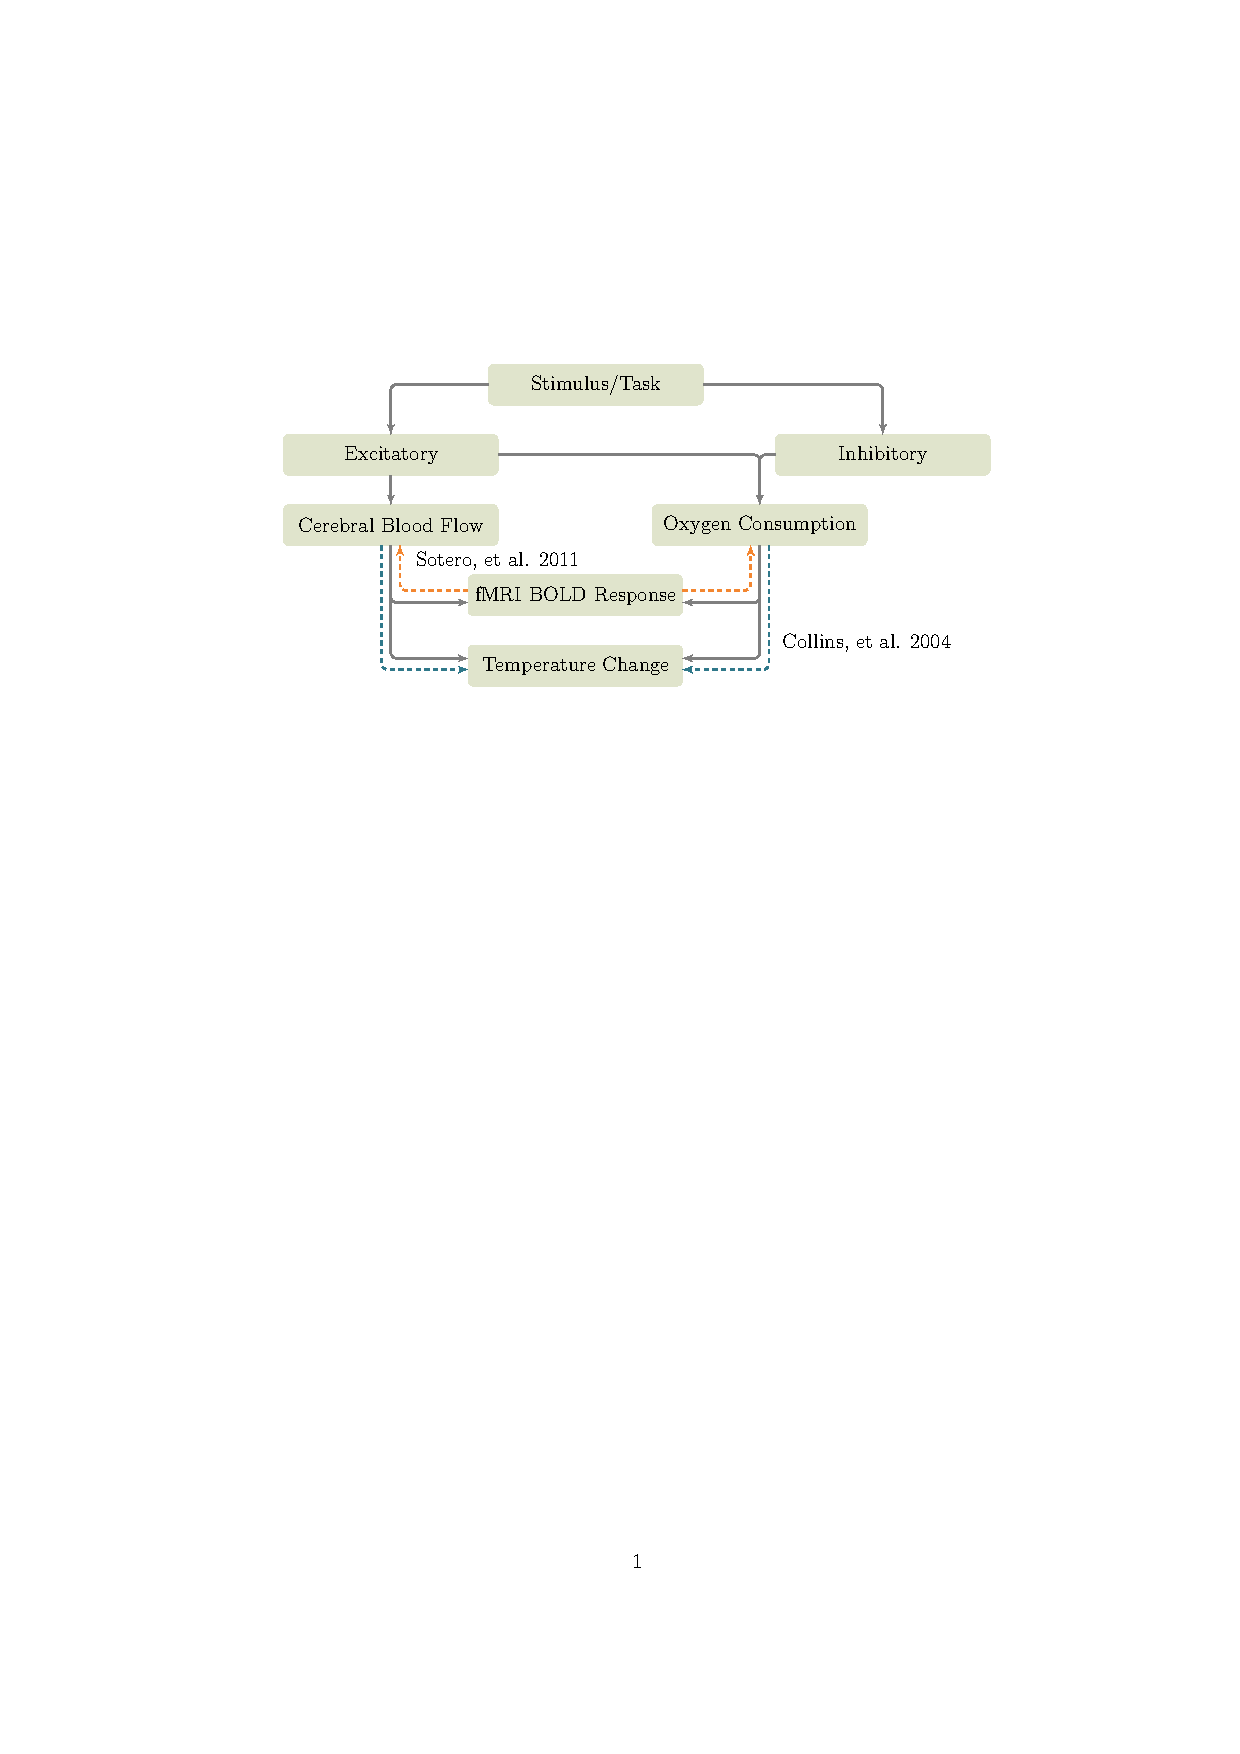
\includegraphics{flowchart}
        \caption[Generation of the fMRI BOLD Response]{\label{fig:flowchart} bla bla bla}
      \end{center}
    \end{figure}
  \subsection{Previously Proposed Temperature Models}
    \subsubsection{Single-Voxel Approach}
    \subsubsection{Multi-Voxel Approach}
  


\section{Modeling the BOLD Response}
% Start with Buxton and Friston and build up to how I am calculating the metabolism and blood flow.

\section{Modeling Temperature}
  % go through the other approaches
  \subsection{The Approach}
    \subsubsection{How the temperature is calculated}
    \subsubsection{Calculating the equilibrium temperature}
    \subsubsection{Calculating Metabolism and Blood Flow Changes}
    \subsubsection{Calculating the change in temperature in the active brain}
  \subsection{Results}
    \subsubsection{Using Theoretical BOLD Data}
    \subsubsection{Using Experimental BOLD Data}
  % talk about my approach